
\begin{figure*}[t] 
	\begin{center} 
		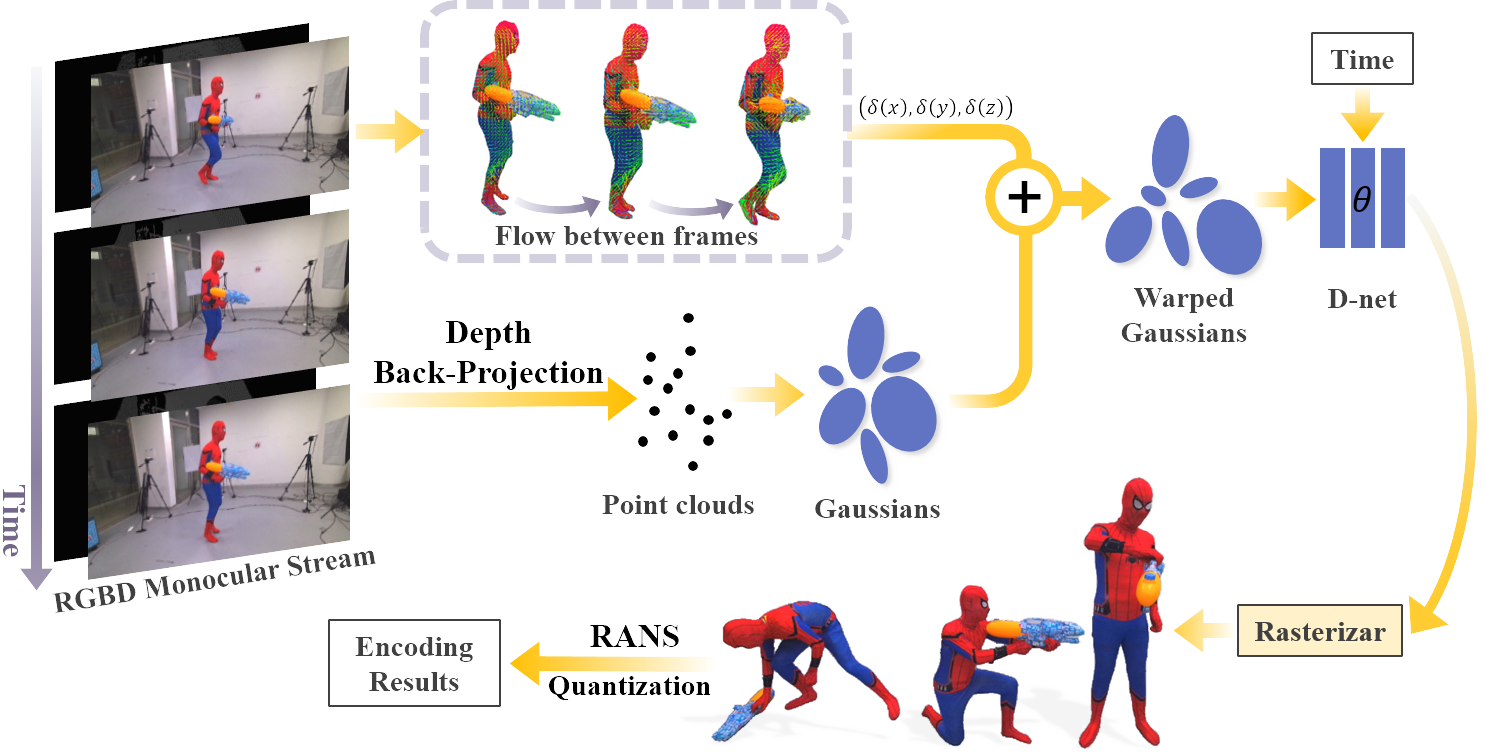
\includegraphics[width=\linewidth]{sec/fig/pipeline.png} 
	\end{center} 
    \vspace{-20pt}  
% (a)我们的setting是RGBD monocular stream (b)对depth反投影产生初始点云初始化gaussians (c)利用flow between frames对gaussians进行warp,得到的warped gaussians作为先验进入deformable net(D-net)(d)D-net额外引入time作为输入估计当前的deltax,deltay,deltaz,deltar (e)对得到的gaussians利用RANS和quantization进行压缩
    \caption{\noindent{\bf Overview of DynTCG.} (a) Our setting involves an RGBD monocular stream. (b) DynTCG performs back-projection on the depth to generate initial point clouds and initialize Gaussians. (c) Utilizing the flow between frames, we warp the Gaussians, and the resulting warped Gaussians are used as a prior input into the deformable network (D-net). (d) The D-net additionally introduces time as an input to estimate the current $\delta(x)$, $\delta(y)$, $\delta(z)$, and $\delta(r)$. (e) After training, the Gaussians are then compressed using RANSAC and quantization.}
	\label{fig:fig_2_overview} 
	\vspace{-8pt}
\end{figure*} 


\section{Introduction}
The precise reconstruction and photorealistic rendering of dynamic scenes from a collection of input images are paramount for numerous applications, such as augmented reality/virtual reality (AR/VR) and 3D content production. In these contexts, achieving high-quality results is essential for an immersive and visually convincing experience. 

% The original radiance methods such as NeRF methods usually have the slower training and rendering speed with with equivalent quality, so the Gaussian-splatting technique was introduced to improve training efficiency, achieved the balance between speed and quantity.
However, the multi-view setting remains impractical for everyday consumer use. In contrast, the monocular method, utilizing a single and convenient commercial RGBD camera, proves to be more practical and appealing for daily applications.

Recent advancements in neural rendering, exemplified by Neural Radiance Fields (NeRF)\cite{mildenhall2020nerf}, have facilitated photorealistic rendering with dense-view supervision. Particularly noteworthy are dynamic variants of NeRF~\cite{gao2021dynamic}, which excel in synthesizing compelling novel views of dynamic scenes, even when captured monocularly. However, these approaches depend on laborious and time-consuming per-scene training to seamlessly integrate temporal observations into the canonical space.

The recent development known as 3D Gaussian Splatting (3DGS) 
~\cite{kerbl3Dgaussians} reverts to an explicit paradigm for representing static scenes. Utilizing GPU-friendly rasterization of 3D Gaussian primitives, it enables real-time and high-quality rendering of radiance fields that were unprecedented until now.

In this paper, we propose DynTCG, a novel approach for synthesizing novel views of dynamic scenes based on flow-tracked and compact Gaussian representations, utilizing monocular dynamic RGBD input. Our key idea involves leveraging the powerful prior provided by flow tracking of 2D images and depth information as the deform field for dynamic Gaussians. Simultaneously, we discovered that optimizing the scaling of Gaussians in the deform-net has minimal impact on appearance and can even affect training speed. Consequently, we modified the deform-net, originally designed in the baseline to optimize position, rotation, and scaling simultaneously. The adjustment now focuses solely on optimizing position and rotation. This alteration aims to enhance training speed with almost negligible impact on rendering quality. Given the substantial storage overhead associated with Gaussians (requiring storage of 3rd-order spherical harmonics coefficients for each point and information for modeling Gaussian scale, position, rotation, and opacity), we introduce a quantization and entropy encoding-based residual compression method tailored for dynamic scenes. This approach transforms the representation of Gaussians into a more compact form, thereby significantly reducing storage requirements.





To summarize, our main contributions include:
 
\begin{itemize}
    \item We propose a deformable Gaussian representation based on 
monocular RGBD input, aimed at accomplishing the task of 
dynamic novel view synthesis.
    \item We observed that optimizing scaling in the deform-net doesn't significantly impact the final rendering of dynamic scenes. On the contrary, it tends to affect training speed. Therefore, we have removed the optimization of scaling from the deform-net。
    \item Utilizing optical flow tracking from 2D images, we provide an 
optimized initialization for the dynamic Gaussian deform field, 
significantly accelerating the training speed and enhancing 
the rendering quality under a monocular setting.
    \item We showcase a companion compression scheme, 
supporting high-quality rendering with low storage, even 
under various platforms.
\end{itemize}

Our method achieves less training time, better rendering quantity, and less per-frame storage, which greatly balances the time consumption and the rendering quality.

